%% Part of Stellarium User Guide
%% Status: 2015-12-30 Some parts collected from wiki.
%%         2016-04-05 GZ changed to have 1 chapter per plugin for a better structure. This file may be split up later. 
%% TODO: All plugins! And give a better structure than just by alphabet.

\chapter{Object Catalog Plugins}
Several plugins provide users with some more object classes. 


\section{Bright Novae Plugin}
\label{sec:plugins:BrightNovae}

\begin{figure}[ht]
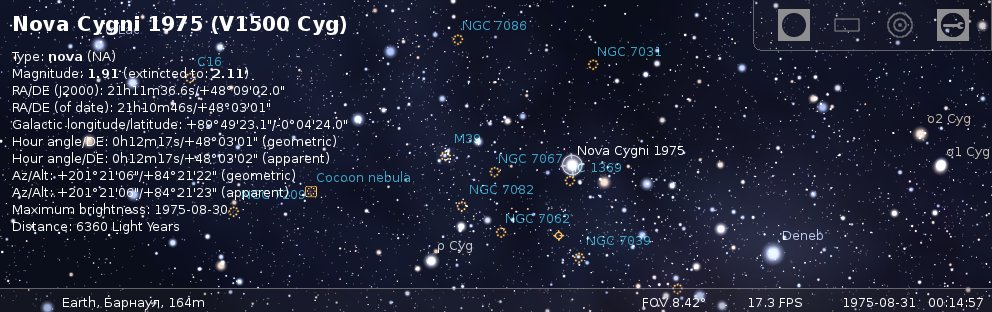
\includegraphics[width=\textwidth]{NovaCygni1975wiki.jpg}
\caption{Nova Cygni 1975 (also known as \textbf{V1500 Cyg})}
\label{fig:NovaCygni1975}
\end{figure}


\noindent The Bright Novae plugin provides visualization of some
bright novae in the Milky Way galaxy.
If enabled (see section~\ref{sec:Plugins:EnablingPlugins}), bright
novae from the past will be presented in the sky at the correct
times. For example, set date and time to 30 August 1975, look at the constellation \emph{Cygnus} to see
\emph{Nova Cygni 1975}\footnote{\url{http://en.wikipedia.org/wiki/V1500_Cygni}} (Fig.~\ref{fig:NovaCygni1975}).


\subsection{Section \big[Novae\big] in config.ini file}
\label{sec:plugins:BrightNovae:config}

You can edit \file{config.ini} file by yourself for changes of the
settings for the Bright Novae plugin -- just make it carefully!

\begin{longtabu} to \textwidth {l|l|X}\toprule
\emph{ID}            & \emph{Type} & \emph{Description}\\\midrule
last\_update            & string & Date and time of last update\\\midrule
update\_frequency\_days & int    & Frequency of updates, in days\\\midrule
updates\_enable         & bool   & Enable updates of bright novae catalog from Internet \\\midrule
url                     & string & URL of bright novae catalog \\\bottomrule
\end{longtabu}

\subsection{Format of bright novae catalog}
\label{sec:plugins:BrightNovae:format}

To add a new nova, open a new line after line 5 and paste the following, note commas and brackets, they are important:

\begin{configfile}
"Nova designation":
{
    "name": "name of nova",
    "type": "type of nova",
    "maxMagnitude": value of maximal visual magnitude,
    "minMagnitude": value of minimal visual magnitude,
    "peakJD": JD for maximal visual magnitude,
    "m2": Time to decline by 2mag from maximum (in days),
    "m3": Time to decline by 3mag from maximum (in days),
    "m6": Time to decline by 6mag from maximum (in days),
    "m9": Time to decline by 9mag from maximum (in days),
    "distance": value of distance between nova and 
                Earth (in thousands of Light Years),
    "RA": "Right ascension (J2000)",
    "Dec": "Declination (J2000)"
},
\end{configfile}

\noindent For example, the record for \textbf{Nova Cygni 1975} (\textbf{V1500 Cyg}) looks like:
\begin{configfile}
"V1500 Cyg":
{
    "name": "Nova Cygni 1975",
    "type": "NA",
    "maxMagnitude": 1.69,
    "minMagnitude": 21,
    "peakJD": 2442655,
    "m2": 2,
    "m3": 4,
    "m6": 32,
    "m9": 263
    "distance": 6.36,
    "RA": "21h11m36.6s",
    "Dec": "48d09m02s"
},
\end{configfile}

\subsection{Light curves}
\label{sec:plugins:BrightNovae:lightcurves}

This plugin uses a very simple model for calculation of light curves for
novae stars. This model is based on time for decay by $N$
magnitudes from the maximum value, where $N$ is 2, 3, 6 and 9. If a
nova has no values for decay of magnitude then this plugin will use
generalized values for it.

\newpage

\section{Historical Supernovae Plugin}
\label{sec:plugins:HistoricalSupernovae}

\begin{figure}[ht]
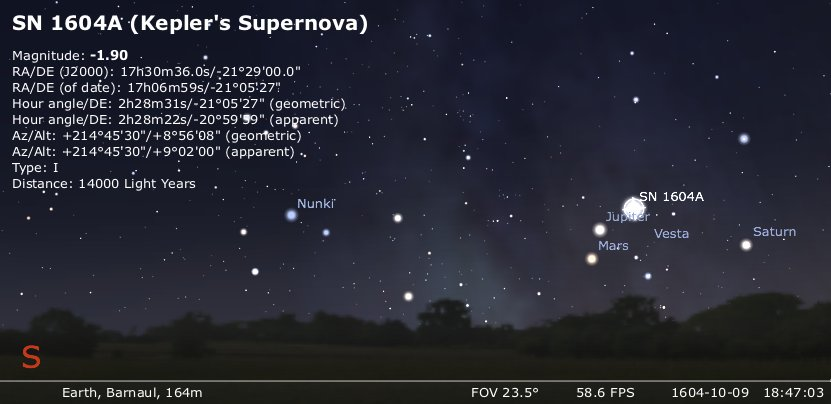
\includegraphics[width=\textwidth]{sn1604wiki.jpg}
\caption{Supernova 1604 (also known as \textbf{Kepler's Supernova}, \textbf{Kepler's Nova} or \textbf{Kepler's Star})}
\label{fig:SN1604}
\end{figure}


\noindent Similar to the Historical Novae plugin
(section~\ref{sec:plugins:BrightNovae}), the Historical Supernovae
plugin provides visualization of bright historical supernovae
(Fig.~\ref{fig:SN1604}) from the table below.
If enabled (see section~\ref{sec:Plugins:EnablingPlugins}), bright
supernovae from the past will be presented in the sky at the correct
times. For example, set date and time to 29 April 1006, and look at the constellation \emph{Lupus} to see \emph{SN 1006A}.


\subsection{List of supernovae in default catalog}
\label{sec:plugins:HistoricalSupernovae:list}


\begin{longtabu} to \textwidth {l|l|l|l|X}\toprule
\emph{Supernova}            & \emph{Date of max. brightness} & \emph{Max. apparent mag.} & \emph{Type} & \emph{Name} \\\midrule
SN 185A\footnote{\url{https://en.wikipedia.org/wiki/SN_185}} & 7 December & -6.0 & Ia & \\\midrule
SN 386A & 24 April & 1.5 & II & \\\midrule
SN 1006A\footnote{\url{https://en.wikipedia.org/wiki/SN_1006}} & 29 April & -7.5 & I & \\\midrule
SN 1054A\footnote{\url{https://en.wikipedia.org/wiki/SN_1054}} & 3 July & -6.0 & II & \\\midrule
SN 1181A\footnote{\url{https://en.wikipedia.org/wiki/SN_1181}} & 4 August & -2.0 & II & \\\midrule
SN 1572A\footnote{\url{https://en.wikipedia.org/wiki/SN_1572}} & 5 November & -4.0 & I & Tycho's Supernova\\\midrule
SN 1604A\footnote{\url{https://en.wikipedia.org/wiki/SN_1604}} & 8 October & -2.0 & I & Kepler's Supernova\\\midrule
SN 1680A\footnote{\url{https://en.wikipedia.org/wiki/Cassiopeia_A}} & 15 August & 6.0 & IIb & Cassiopeia A\\\midrule
SN 1885A\footnote{\url{https://en.wikipedia.org/wiki/S_Andromedae}} & 17 August & 5.8 & IPec & S Andromedae\\\midrule
SN 1895B & 5 July & 8.0 & I & \\\midrule
SN 1920A & 17 December & 11.7 & II & \\\midrule
SN 1921C & 11 December & 11.0 & I & \\\midrule
SN 1937C & 21 August & 8.5 & Ia & \\\midrule
SN 1960F & 21 April & 11.6 & Ia & \\\midrule
SN 1960R & 19 December & 12.0 & I & \\\midrule
SN 1961H & 8 May & 11.8 & Ia & \\\midrule
SN 1962M & 26 November & 11.5 & II & \\\midrule
SN 1966J & 2 December & 11.3 & I & \\\midrule
SN 1968L & 12 July & 11.9 & IIP & \\\midrule
SN 1970G & 30 July & 11.4 & IIL & \\\midrule
SN 1971I & 29 May & 11.9 & Ia & \\\midrule
SN 1972E\footnote{\url{https://en.wikipedia.org/wiki/SN1972e}} & 8 May & 8.4 & Ia & \\\midrule
SN 1979C & 15 April & 11.6 & IIL & \\\midrule
SN 1980K & 31 October & 11.6 & IIL & \\\midrule
SN 1981B & 9 March & 12.0 & Ia & \\\midrule
SN 1983N & 17 July & 11.4 & Ib & \\\midrule
SN 1987A\footnote{\url{https://en.wikipedia.org/wiki/SN_1987A}} & 24 February & 2.9 & IIPec & \\\midrule
SN 1989B & 6 February & 11.9 & Ia & \\\midrule
SN 1991T & 26 April & 11.6 & IaPec & \\\midrule
SN 1993J\footnote{\url{https://en.wikipedia.org/wiki/SN_1993J}} & 30 March & 10.8 & IIb & \\\midrule
SN 1994D & 31 March & 11.8 & Ia & \\\midrule
SN 1998bu & 21 May & 11.9 & Ia & \\\midrule
SN 2004dj & 31 July & 11.3 & IIP & \\\midrule
SN 2011fe\footnote{\url{https://en.wikipedia.org/wiki/SN_2011fe}} & 13 September & 10.06 & Ia & \\\midrule
SN 2013aa & 13 February	& 11.9 & Ia & \\\bottomrule
\end{longtabu}

\subsection{Light curves}
\label{sec:plugins:HistoricalSupernovae:lightcurves}

In this plugin a simple model of light curves for different supernovae
has been implemented. A typical light curve used in the plugin for
supernova type~I is shown in Fig.~\ref{fig:SNTypeI} (bottom scale in
days).

\begin{figure}[ht]
\begin{center}
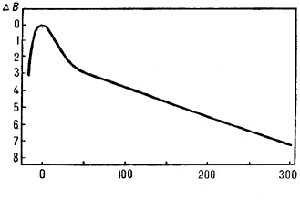
\includegraphics[width=250px]{sn_type_I.jpg}
\end{center}
\caption{Light Curve of Supernova Type I}
\label{fig:SNTypeI}
\end{figure}

For supernova type~II we use a typical light curve with plateau, which
you can see in Fig.~\ref{fig:SNTypeII} (bottom scale in days).

\begin{figure}[ht]
\begin{center}
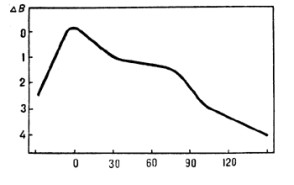
\includegraphics[width=260px]{sn_type_II.jpg}
\end{center}
\caption{Light Curve of Supernova Type II}
\label{fig:SNTypeII}
\end{figure}

In both images for light curves the maximum brightness is marked as day 0.

\subsection{Section \big[Supernovae\big] in config.ini file}
\label{sec:plugins:HistoricalSupernovae:config}

You can edit \file{config.ini} file by yourself for changes of the
settings for the Historical Supernovae plugin -- just make it carefully!

\begin{longtabu} to \textwidth {l|l|X}\toprule
\emph{ID}            & \emph{Type} & \emph{Description}\\\midrule
last\_update            & string & Date and time of last update\\\midrule
update\_frequency\_days & int    & Frequency of updates, in days\\\midrule
updates\_enable         & bool   & Enable updates of bright novae catalog from Internet \\\midrule
url                     & string & URL of bright novae catalog \\\bottomrule
\end{longtabu}

\newpage
\subsection{Format of historical supernovae catalog}
\label{sec:plugins:HistoricalSupernovae:format}

To add a new nova, open a new line after line 5 and paste the following, note commas and brackets, they are important:

\begin{configfile}
"Supernova designation":
{
    "type": "type of supernova",
    "maxMagnitude": value of maximal visual magnitude,
    "peakJD": JD for maximal visual magnitude,
    "alpha": "Right ascension (J2000)",
    "delta": "Declination (J2000)",
    "distance": value of distance between supernova and 
                Earth (in thousands of Light Years),
    "note": "notes for supernova"
},
\end{configfile}

\noindent For example, the record for \textbf{SN 1604A} (\textbf{Kepler's Supernova}) looks like:
\begin{configfile}
"1604A":
{
    "type": "I",
    "maxMagnitude": -2,
    "peakJD": 2307190,
    "alpha": "17h30m36.00s",
    "delta": "-21d29m00.0s",
    "distance": 14,
    "note": "Kepler's Supernova"
},
\end{configfile}

\newpage

\section{Exoplanets Plugin}
\label{sec:plugins:Exoplanets}

\begin{figure}[h]
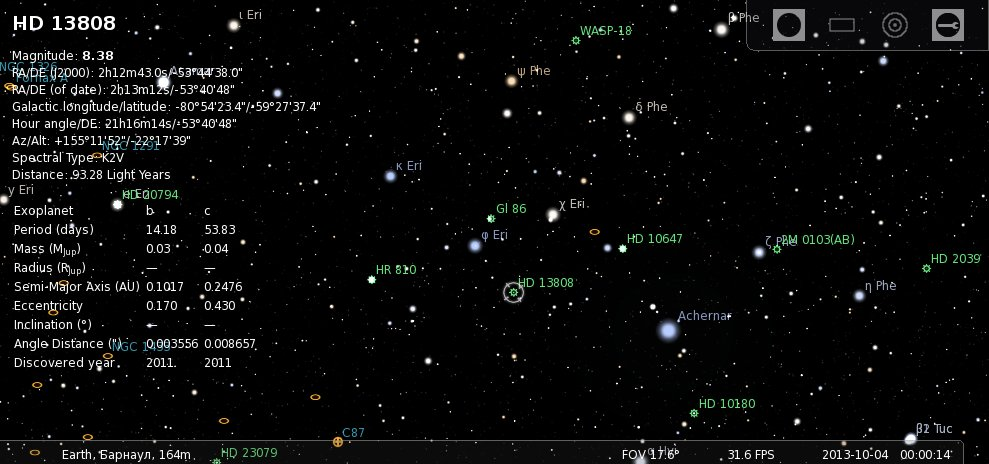
\includegraphics[width=\textwidth]{exoplanets.jpg}
\caption{Planetary system HD 13808}
\label{fig:Exoplanets}
\end{figure}

\noindent This plugin plots the position of stars with
exoplanets. Exoplanets data is derived from ``The Extrasolar Planets
Encyclopaedia''\footnote{\url{http://exoplanet.eu/}}. List of
potential habitable exoplanets and data about them were taken from
``The Habitable Exoplanets
Catalog''\footnote{\url{http://phl.upr.edu/projects/habitable-exoplanets-catalog}}
by the Planetary Habitability
Laboratory\footnote{\url{http://phl.upr.edu/home}}.  If enabled (see
section~\ref{sec:Plugins:EnablingPlugins}), just click on the
Exoplanet button \guibutton{0.6}{btExoplanets-off} on the bottom
toolbar to display markers for the stars with known exoplanets. You
can then either click on such a marked star or find the stars with
exoplanets by their designation (e.g., \emph{24 Sex}) in the \key{F3} dialog (see~\ref{sec:gui:search}).


\subsection{Potential habitable exoplanets}
\label{sec:plugins:Exoplanets:habitable}
This plugin can display potential habitable exoplanets (orange marker) and some information about those planets.

\begin{description}
\item[Planetary Class] Planet classification from host star spectral
  type (F, G, K, M; see
  section~\ref{sec:Phenomena:SpectralTypeLuminosityClass}), habitable
  zone (hot, warm, cold) and size (miniterran, subterran, terran,
  superterran, jovian, neptunian) (Earth = G-Warm Terran).
\item[Equilibrium Temperature] The planetary equilibrium
  temperature\footnote{\url{http://lasp.colorado.edu/~bagenal/3720/CLASS6/6EquilibriumTemp.html}}
  is a theoretical temperature (in \degree C) that the planet would be
  at when considered simply as if it were a black body being heated
  only by its parent star (assuming a 0.3 bond albedo). As example the
  planetary equilibrium temperature of Earth is -18.15\degree C (255~K).
\item[Earth Similarity Index (ESI)] Similarity to
  Earth\footnote{\url{http://phl.upr.edu/projects/earth-similarity-index-esi}}
  on a scale from 0 to 1, with 1 being the most Earth-like. ESI
  depends on the planet's radius, density, escape velocity, and
  surface temperature.
\end{description}

\subsection{Proper names}
\label{sec:plugins:Exoplanets:ProperNames}
In December 2015, the International Astronomical Union (IAU) has officially approved names for several exoplanets after a public vote.
\begin{description}
\item[Veritate]* (14 And) -- From the latin Veritas, truth. The ablative form means \textit{where there is truth}\footnote{The original name proposed, Veritas, is that of an asteroid important for the study of the solar system.}.
\item[Spe]* (14 And b) -- From the latin Spes, hope. The ablative form means \textit{where there is hope}.
\item[Musica] (18 Del) -- Musica is Latin for \textit{music}.
\item[Arion] (18 Del b) -- Arion was a genius of poetry and music in ancient Greece. According to legend, his life was saved at sea by dolphins after attracting their attention by the playing of his kithara.
\item[Fafnir] (42 Dra) -- Fafnir was a Norse mythological dwarf who turned into a dragon.
\item[Orbitar] (42 Dra b) -- Orbitar is a contrived word paying homage to the space launch and orbital operations of NASA.
\item[Chalawan] (47 UMa) -- Chalawan is a mythological crocodile king from a Thai folktale.
\item[Taphao Thong] (47 UMa b) -- Taphao Thong is one of two sisters associated with the Thai folk tale of Chalawan.
\item[Taphao Kaew] (47 UMa c) -- Taphao Kae is one of two sisters associated with the Thai folk tale of Chalawan.
\item[Helvetios] (51 Peg) -- Helvetios is Celtic for the \textit{Helvetian} and refers to the Celtic tribe that lived in Switzerland during antiquity.
\item[Dimidium] (51 Peg b) -- Dimidium is Latin for \textit{half}, referring to the planet's mass of at least half the mass of Jupiter.
\item[Copernicus] (55 Cnc) -- Nicolaus Copernicus or Mikolaj Kopernik (1473-1543) was a Polish astronomer who proposed the heliocentric model of the solar system in his book ``De revolutionibus orbium coelestium''.
\item[Galileo] (55 Cnc b) -- Galileo Galilei (1564-1642) was an Italian astronomer and physicist often called the \textit{father of observational astronomy} and the \textit{father of modern physics}. Using a telescope, he discovered the four largest satellites of Jupiter, and the reported the first telescopic observations of the phases of Venus, among other discoveries.
\item[Brahe] (55 Cnc c) -- Tycho Brahe (1546-1601) was a Danish astronomer and nobleman who recorded accurate astronomical observations of the stars and planets. These observations were critical to Kepler's formulation of his three laws of planetary motion.
\item[Lipperhey]* (55 Cnc d) -- Hans Lipperhey (1570-1619) was a German-Dutch lens grinder and spectacle maker who is often attributed with the invention of the refracting telescope in 1608\footnote{The original spelling of Lippershey was corrected to Lipperhey on 15.01.2016. The commonly seen spelling Lippershey (with an s) results in fact from a typographical error dating back from 1831, thus should be avoided.}.
\item[Janssen] (55 Cnc e) -- Jacharias Janssen (1580s-1630s) was a Dutch spectacle maker who is often attributed with invention of the microscope, and more controversially with the invention of the telescope.
\item[Harriot] (55 Cnc f) -- Thomas Harriot (ca. 1560-1621) was an English astronomer, mathematician, ethnographer, and translator, who is attributed with the first drawing of the Moon through telescopic observations.
\item[Amateru]* ($\epsilon$ Tau b) -- \textit{Amateru} is a common Japanese appellation for shrines when they enshrine Amaterasu, the Shinto goddess of the Sun, born from the left eye of the god Izanagi\footnote{The name originally proposed, Amaterasu, is already used for an asteroid.}.
\item[Hypatia] ($\iota$ Dra b) -- Hypatia was a famous Greek astronomer, mathematician, and philosopher. She was head of the Neo-Platonic school at Alexandria in the early 5th century, until murdered by a Christian mob in 415.
\item[Ran]* ($\epsilon$ Eri) -- Ran is the Norse goddess of the sea, who stirs up the waves and captures sailors with her net.
\item[AEgir]* ($\epsilon$ Eri b) -- AEgir is Ran's husband, the personified god of the ocean. \textit{AEgir} and \textit{Ran} both represent the \textit{Jotuns} who reign in the outer Universe; together they had nine daughters\footnote{Note the typographical difference between AEgir and Aegir, the Norwegian transliteration. The same name, with the spelling Aegir, has been attributed to one of Saturn's satellites, discovered in 2004.}.
\item[Tadmor]* ($\gamma$ Cep b) -- Ancient Semitic name and modern Arabic name for the city of Palmyra, a UNESCO World Heritage Site.
\item[Dagon] ($\alpha$ PsA b) -- Dagon was a Semitic deity, often represented as half-man, half-fish.
\item[Tonatiuh] (HD 104985) -- Tonatiuh was the Aztec god of the Sun.
\item[Meztli] (HD 104985 b) -- Meztli was the Aztec goddess of the Moon.
\item[Ogma]* (HD 149026) -- Ogma was a deity of eloquence, writing, and great physical strength in the Celtic mythologies of Ireland and Scotland, and may be related to the Gallo-Roman deity \textit{Ogmios}\footnote{Ogmios is a name already attributed to an asteroid.}.
\item[Smertrios] (HD 149026 b) -- Smertrios was a Gallic deity of war.
\item[Intercrus] (HD 81688) -- Intercrus means \textit{between the legs} in Latin style, referring to the star's position in the constellation Ursa Major.
\item[Arkas] (HD 81688 b) -- Arkas was the son of Callisto (Ursa Major) in Greek mythology.
\item[Cervantes] ($\mu$ Ara) -- Miguel de Cervantes Saavedra (1547-1616) was a famous Spanish writer and author of ``El Ingenioso Hidalgo Don Quixote de la Mancha''.
\item[Quijote] ($\mu$ Ara b) -- Lead fictional character from Cervantes's ``El Ingenioso Hidalgo Don Quixote de la Mancha''.
\item[Dulcinea]($\mu$ Ara c) — Fictional character and love interest of Don Quijote (or Quixote) in Cervantes's ``El Ingenioso Hidalgo Don Quixote de la Mancha''.
\item[Rocinante] ($\mu$ Ara d) -- Fictional horse of Don Quijote in Cervantes's ``El Ingenioso Hidalgo Don Quixote de la Mancha''.
\item[Sancho] ($\mu$ Ara e) -- Fictional squire of Don Quijote in Cervantes's ``El Ingenioso Hidalgo Don Quixote de la Mancha''.
\item[Thestias]* ($\beta$ Gem b) -- Thestias is the patronym of Leda and her sister Althaea, the daughters of Thestius. Leda was a Greek queen, mother of Pollux and of his twin Castor, and of Helen and Clytemnestra\footnote{The original proposed name Leda is already attributed to an asteroid and to one of Jupiter's satellites. The name Althaea is also attributed to an asteroid.}.
\item[Lich] (PSR B1257+12) -- Lich is a fictional undead creature known for controlling other undead creatures with magic.
\item[Draugr] (PSR B1257+12 b) -- Draugr refers to undead creatures in Norse mythology.
\item[Poltergeist] (PSR B1257+12 c) -- Poltergeist is a name for supernatural beings that create physical disturbances, from German for noisy ghost.
\item[Phobetor] (PSR B1257+12 d) -- Phobetor is a Greek mythological deity of nightmares, the son of Nyx, the primordial deity of night.
\item[Titawin] ($\upsilon$ And) -- Titawin (also known as Medina of Tetouan) is a settlement in northern Morocco and UNESCO World Heritage Site. Historically it was an important point of contact between two civilizations (Spanish and Arab) and two continents (Europe and Africa) after the $8^{th}$ century.
\item[Saffar] ($\upsilon$ And b) -- Saffar is named for Abu al-Qasim Ahmed Ibn-Abd Allah Ibn-Omar al Ghafiqi Ibn-al-Saffar, who taught arithmetic, geometry, and astronomy in 11th century Cordova in Andalusia (modern Spain), and wrote an influential treatise on the uses of the astrolabe.
\item[Samh] ($\upsilon$ And c) -- Samh is named for Abu al-Qasim 'Asbagh ibn Muhammad ibn al-Samh al-Mahri (or Ibn al-Samh), a noted 11th century astronomer and mathematician in the school of al Majriti in Cordova (Andalusia, now modern Spain).
\item[Majriti] ($\upsilon$ And d) -- Majriti is named for Abu al-Qasim al-Qurtubi al-Majriti, a notable mathematician, astronomer, scholar, and teacher in $10^{th}$ century and early $11^{th}$ century Andalusia (modern Spain).
\item[Libertas]* ($\xi$ Aql) -- Libertas is Latin for liberty. Liberty refers to social and political freedoms, and a reminder that there are people deprived of liberty in the world even today. The constellation Aquila represents an eagle -- a popular symbol of liberty.
\item[Fortitudo]* ($\xi$ Aql b) -- Fortitudo is Latin for fortitude. Fortitude means emotional and mental strength in the face of adversity, as embodied by the eagle (represented by the constellation Aquila).
\end{description}

All names with asterix mark (*) are modified based on the original proposals, to be consistent with the IAU rules.


\subsection{Section \big[Exoplanets\big] in config.ini file}
\label{sec:plugins:Exoplanets:config}

You can edit \file{config.ini} file by yourself for changes of the
settings for the Exoplanets plugin -- just make it carefully!

\begin{longtabu} to \textwidth {l|l|X}\toprule
\emph{ID}            & \emph{Type} & \emph{Description}\\\midrule
last\_update  & string & Date and time of last update \\\midrule
update\_frequency\_hours  & int & Frequency of updates, in hours \\\midrule
updates\_enable  & bool & Enable updates of exoplanets catalog from Internet \\\midrule
url  & string & URL of exoplanets catalog \\\midrule
flag\_show\_exoplanets\_button  & bool & Enable showing button of exoplanets on bottom bar \\\midrule
distribution\_enabled  & bool & Enable distribution mode of display \\\midrule
timeline\_enabled  & bool & Enable timeline mode of display \\\midrule
habitable\_enabled  & bool & Enable habitable mode of display \\\midrule
enable\_at\_startup  & bool & Enable displaying exoplanets at startup of the plugin \\\midrule
exoplanet\_marker\_color & R,G,B & Color for marker of star with planetary system \\\midrule
habitable\_exoplanet\_marker\_color  & R,G,B & Color for marker of star with planetary system with potential habitable exoplanets
 \\\bottomrule
\end{longtabu}

\newpage
\subsection{Format of exoplanets catalog}
\label{sec:plugins:Exoplanets:format}

To add a new exoplanet system, open a new line after line 5 and paste the following, note commas and brackets, they are important:

\begin{configfile}
"Star designation":
{
	"exoplanets":
	[
	{
		"mass": mass of exoplanet (M jup),
		"radius": radius of exoplanet (R jup),
		"period": period of exoplanet (days),
		"semiAxis": semi-major axis (AU),
		"eccentricity": orbit's eccentricity,
		"inclination": orbit's inclination (degree),
		"angleDistance": angle distance from star 
		                 (arcseconds),
		"discovered": exoplanet discovered year,
		"hclass": "habitable class",
		"MSTemp": mean surface temperature (K),
		"ESI": Earth Similarity Index (*100),
		"planetProperName": "proper name of planet",
		"planetName": "designation of planet"
	},
	{
		"mass": mass of exoplanet (M jup),
		"radius": radius of exoplanet (R jup),
		"period": period of exoplanet (days),
		"semiAxis": semi-major axis (AU),
		"eccentricity": orbit's eccentricity,
		"inclination": orbit's inclination (degree),
		"angleDistance": angle distance from star 
		                 (arcseconds),
		"discovered": exoplanet discovered year,
		"hclass": "habitable class",
		"MSTemp": mean surface temperature (K),
		"ESI": Earth Similarity Index (*100),
		"planetProperName": "proper name of planet",
		"planetName": "designation of planet"
	}
	],
	"distance": value of distance to star (pc),
	"stype": "spectral type of star",
	"smass": value of mass of star (M sun),
	"smetal": value of metallicity of star,
	"Vmag": value of visual magnitude of star,
	"sradius": value of radius of star (R sun),
	"effectiveTemp": value of effective temperature 
	                 of star (K),
	"starProperName": "proper name of the star",
	"hasHP": boolean (has potential habitable planets),
	"RA": "Right ascension (J2000)",
	"DE": "Declination (J2000)"
},
\end{configfile}

\noindent For example, the record for \textit{24 Sex} looks like:
\begin{configfile}
"24 Sex":
{
		"exoplanets":
		[
		{
			"mass": 1.99,
			"period": 452.8,
			"semiAxis": 1.333,
			"eccentricity": 0.09,
			"angleDistance": 0.017821,
			"discovered": 2010,
			"planetName": "b"
		},
		{
			"mass": 0.86,
			"period": 883.0,
			"semiAxis": 2.08,
			"eccentricity": 0.29,
			"angleDistance": 0.027807,
			"discovered": 2010,
			"planetName": "c"
		}
		],
		"distance": 74.8,
		"stype": "G5",
		"smass": 1.54,
		"smetal": -0.03,
		"Vmag": 7.38,
		"sradius": 4.9,
		"effectiveTemp": 5098,
		"RA": "10h23m28s",
		"DE": "-00d54m08s"
},
\end{configfile}


\newpage

\section{Pulsars Plugin}
\label{sec:plugins:Pulsars}

\begin{figure}[ht]
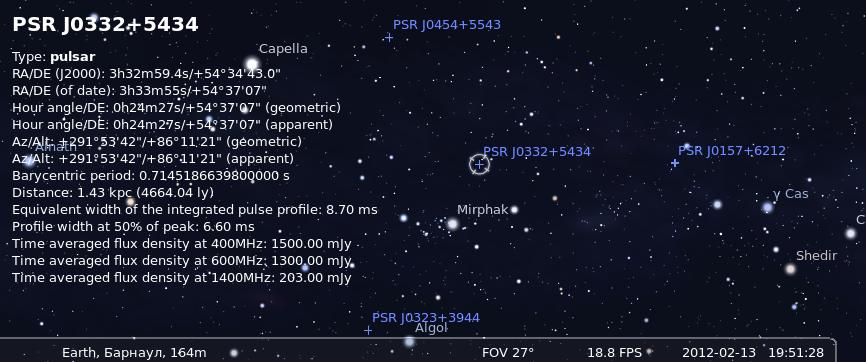
\includegraphics[width=\textwidth]{psr_j0332_5434.jpg}
\caption{PSR J0332-5434}
\label{fig:plugin:Pulsars}
\end{figure}

\noindent This plugin plots the position of various pulsars, with object
information about each one. Pulsar data is derived from \textit{The
  ATNF Pulsar Catalogue} \cite{2005AJ....129.1993M}.

If enabled (see section~\ref{sec:Plugins:EnablingPlugins}), use the
\guibutton{0.6}{btPulsars-off} button to activate display of
pulsars. The GUI allows a few configuration options.  You can also
find a pulsar (\key{F3}) by its designation (e.g., \emph{PSR
  J0437-4715}).



\subsection{Section \big[Pulsars\big] in config.ini file}
\label{sec:plugins:Pulsars:config}

\begin{longtabu} to \textwidth {l|l|X}\toprule
\emph{ID}               & \emph{Type} & \emph{Description}\\\midrule
last\_update                & string & Date and time of last update\\\midrule
update\_frequency\_days     & int    & Frequency of updates, in days\\\midrule
updates\_enable             & bool   & Enable updates of pulsars catalog from Internet \\\midrule
url                         & string & URL of pulsars catalog \\\midrule
enable\_at\_startup         & bool   & Enable displaying of pulsars at startup of Stellarium \\\midrule
distribution\_enabled       & bool   & Enable distribution mode for the pulsars \\\midrule
flag\_show\_pulsars\_button & bool   & Enable displaying pulsars button on toolbar \\\midrule
marker\_color               & R,G,B  & Color for marker of the pulsars \\\midrule
glitch\_color               & R,G,B  & Color for marker of the pulsars with glitches \\\midrule
use\_separate\_colors       & bool   & Use separate colors for different types of the pulsars \\\bottomrule
\end{longtabu}

\newpage
\subsection{Format of pulsars catalog}
\label{sec:plugins:Pulsars:format}

To add a new pulsar, open a new line after line 5 and paste the following, note commas and brackets, they are important:

\begin{configfile}
"Pulsar designation":
{
    "RA": "Right ascension (J2000)",
    "DE": "Declination (J2000)",
    "notes": "type of pulsar",
    "distance": value of distance based on electron density 
                model (kpc),
    "period": value of barycentric period of the pulsar (s),
    "parallax": value of annular parallax (mas),
    "bperiod": value of binary period of pulsar (days),
    "pderivative": value of time derivative of barcycentric 
                   period,
    "dmeasure": value of dispersion measure (cm^-3 pc),
    "frequency": value of barycentric rotation frequency (Hz),
    "pfrequency": value of time derivative of barycentric 
                  rotation frequency (s^-2)
    "eccentricity": value of eccentricity,                   
    "w50": value of profile width at 50% of peak (ms),
    "s400": value of time averaged flux density at 
            400 MHz (mJy),
    "s600": value of time averaged flux density at 
            600 MHz (mJy),
    "s1400": value of time averaged flux density at 
             1400 MHz (mJy)    
},
\end{configfile}

%\newpage
\noindent For example, the record for \textbf{PSR J0014+4746} looks like:
\begin{configfile}
"PSR J0014+4746":
{
    "distance": 1.82,
    "dmeasure": 30.85,
    "frequency": 0.805997239145,
    "pfrequency": -3.6669E-16,
    "w50": 88.7,
    "s400": 14,
    "s600": 9,
    "s1400": 3,
    "RA": "00h14m17.75s",
    "DE": "47d46m33.4s"
},
\end{configfile}

\newpage
\section{Quasars Plugin}
\label{sec:plugins:Quasars}

\noindent The Quasars plugin provides visualization of some quasars brighter than 16 visual magnitude. A catalogue of quasars compiled from \textit{Quasars and Active Galactic Nuclei} (13th Ed.) \cite{2010A&A...518A..10V}.

\begin{figure}[ht]
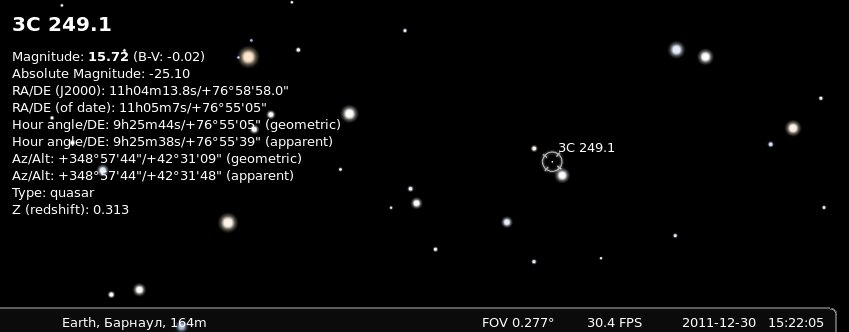
\includegraphics[width=\textwidth]{qso_3c_249_1.jpg}
\caption{3C 249.1, also known as LEDA 2821945 or 4C 77.09}
\label{fig:plugin:Quasars}
\end{figure}


%% TODO follow scheme from Pulsars above. Add a section about QSOs in astornomical phenomena (after galaxies) and add reference from here.


If enabled (see section~\ref{sec:Plugins:EnablingPlugins}), use the
\guibutton{0.6}{btQuasars-off} button to activate display of
quasars. The GUI allows a few configuration options.  You can also
find a quasar (\key{F3}) by its designation (e.g., \emph{3C 273}).

\subsection{Section \big[Quasars\big] in config.ini file}
\label{sec:plugins:Quasars:config}

\begin{longtabu} to \textwidth {l|l|X}\toprule
\emph{ID}               & \emph{Type} & \emph{Description}\\\midrule
last\_update                & string & Date and time of last update\\\midrule
update\_frequency\_days     & int    & Frequency of updates, in days\\\midrule
updates\_enable             & bool   & Enable updates of quasars catalog from Internet \\\midrule
url                         & string & URL of quasars catalog \\\midrule
enable\_at\_startup         & bool   & Enable displaying of quasars at startup of Stellarium \\\midrule
distribution\_enabled       & bool   & Enable distribution mode for the quasars \\\midrule
flag\_show\_quasars\_button & bool   & Enable displaying quasars button on toolbar \\\midrule
marker\_color               & R,G,B  & Color for marker of the quasars \\\bottomrule
\end{longtabu}

\newpage
\subsection{Format of quasars catalog}
\label{sec:plugins:Quasars:format}

To add a new quasar, open a new line after line 5 and paste the following, note commas and brackets, they are important:

\begin{configfile}
"Quasar designation":
{
    "RA": "Right ascension (J2000)",
    "DE": "Declination (J2000)",
    "Amag": value of absolute magnitude,
    "Vmag": value of visual magnitude,
    "z": value of Z (redshift),
    "bV": value of B-V colour
},
\end{configfile}

%\newpage
\noindent For example, the record for \textbf{3C 249.1} looks like:
\begin{configfile}
"3C 249.1":
{
    "RA": "11h04m13.8s",
    "DE": "+76d58m58s",
    "Amag": -25.1,
    "Vmag": 15.72,
    "z": 0.313,
    "bV": -0.02
},
\end{configfile}


\newpage


\section{Meteor Showers Plugin}
\label{sec:plugins:MeteorShowers}

\begin{figure}[ht]
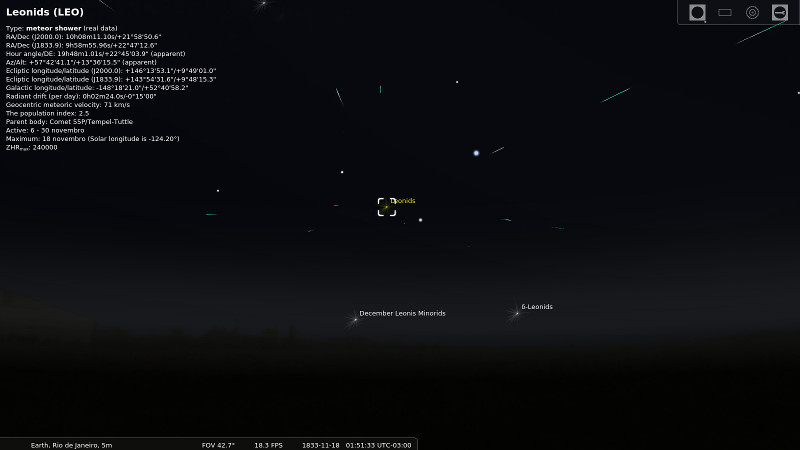
\includegraphics[width=\textwidth]{meteorshowers.jpg}
\caption{The 1833 Leonids replayed with the Meteor Showers plugin.}
\label{fig:plugins:MeteorShowers}
\end{figure}

\noindent In contrast and extension of the random \emph{shooting stars}
feature of Stellarium (see section~\ref{sec:Phenomena:Meteoroids}), this 
plugin provides data for real meteor showers and a marker for each 
active and inactive radiant, showing real information about its activity. 
If enabled (see section~\ref{sec:Plugins:EnablingPlugins}), just click 
on the Meteor Showers button \guibutton{0.6}{btMS-off}  on the bottom
toolbar to display markers for the radiants.


%% TODO: Consider moving to the astronomical phenomena chapter on meteor(oid)s?
\subsection{Terms}
\label{sec:plugins:MeteorShowers:terms}

\paragraph{Meteor shower}
A \indexterm{meteor shower} is a celestial event in which a number of
meteors are observed to radiate, or originate, from one point in the
night sky. These meteors are caused by streams of cosmic debris called
\indexterm{meteoroids} entering Earth's atmosphere at extremely high speeds on
parallel trajectories. Most meteors are smaller than a grain of sand,
so almost all of them disintegrate and never hit the Earth's
surface. Intense or unusual meteor showers are known as meteor
outbursts and meteor storms, which may produce greater than 1,000
meteors an hour.

\paragraph{Radiant}

The \indexterm{radiant} or \indexterm{apparent radiant} of a meteor
shower is the point in the sky from which (to a planetary observer)
meteors appear to originate. The Perseids, for example, are meteors
which appear to come from a point within the constellation of Perseus.

An observer might see such a meteor anywhere in the sky but the
direction of motion, when traced back, will point to the radiant. A
meteor that does not point back to the known radiant for a given
shower is known as a sporadic and is not considered part of that
shower.

Many showers have a radiant point that changes position during the
interval when it appears. For example, the radiant point for the Delta
Aurigids drifts by more than a degree per night.

\paragraph{Zenithal Hourly Rate (ZHR)}

The \indexterm{Zenithal Hourly Rate} (ZHR) of a meteor
shower is the number of meteors a single observer would see in one
hour under a clear, dark sky (limiting apparent magnitude of 6.5) if
the radiant of the shower were at the zenith. The rate that can
effectively be seen is nearly always lower and decreases the closer
the radiant is to the horizon.

\paragraph{Population index}

The \indexterm{population index} indicates the magnitude distribution
of the meteor showers. Values below 2.5 correspond to
distributions where bright meteors are more frequent than average,
while values above 3.0 mean that the share of faint meteors is larger
than usual.

\subsection{Section \big[MeteorShowers\big] in config.ini file}
\label{sec:plugins:MeteorShowers:config}

You can edit \file{config.ini} file by yourself for changes of the
settings for the Meteor Showers plugin~-- just make it carefully!

\begin{longtabu} to \textwidth {l|l|X}\toprule
\emph{ID}            & \emph{Type} & \emph{Description}\\\midrule
last\_update         & string & Date and time of last update \\\midrule
update\_frequency\_hours & int & Frequency of updates, in hours \\\midrule
updates\_enable      & bool & Enable updates of the meteor showers catalog from Internet \\\midrule
url                  & string & URL of the meteor showers catalog \\\midrule
flag\_show\_ms\_button & bool & Enable showing button of the meteor showers on bottom bar \\\midrule
flag\_show\_radiants   & bool & Enable displaying markers for the radiants of the meteor showers \\\midrule
flag\_active\_radiants & bool & Flag for displaying markers for the radiants of the active meteor showers only \\\midrule
enable\_at\_startup    & bool & Enable displaying meteor showers at starup plugin \\\midrule
show\_radiants\_labels & bool & Flag for displaying labels near markers of the radiants of the meteor showers \\\midrule
font\_size             & int  & Font size for label of markers of the radiants of the meteor showers \\\midrule
colorARG               & R,G,B & Color for marker of active meteor showers with generic data \\\midrule
colorARR               & R,G,B & Color for marker of active meteor showers with real data \\\midrule
colorIR               & R,G,B & Color for marker of inactive meteor showers \\\bottomrule
\end{longtabu}

\newpage
\subsection{Format of Meteor Showers catalog}
\label{sec:plugins:MeteorShowers:format}

To add a new meteor shower, you just need to:
\begin{enumerate}
\item Copy the code of some valid meteor shower;
\item Paste it in the line 6 (right after the "showers": \{) of the showers.json document;
\item Replace the information according with your needs.
\end{enumerate}
Note commas and brackets, they are very important! For example, below is a record for \textit{Northern Taurids}:

\begin{configfile}
"NTA":
	{
		"designation": "Northern Taurids",
		"activity":
		[
		{
			"year": "generic",
			"zhr": 5,
			"start": "09.25",
			"finish": "11.25",
			"peak": "11.12"
		},
		{
			"year": "2014",
			"start": "10.20",
			"finish": "12.10"
		},
		{
			"year": "2013",
			"start": "10.20",
			"finish": "12.10"
		},
		{
			"year": "2012",
			"start": "10.20",
			"finish": "12.10"
		},
		{
			"year": "2011",
			"start": "10.20",
			"finish": "12.10"
		}
		],
		"speed": 29,
		"radiantAlpha": "58",
		"radiantDelta": "+22",
		"driftAlpha": "5",
		"driftDelta": "1",
		"colors":
		[
		{
			"color": "yellow",
			"intensity": 80
		},
		{
			"color": "white",
			"intensity": 20
		}
		],
		"parentObj": "Comet C/1917 F1 (Mellish)",
		"pidx": 2.3
	},
\end{configfile}

\subsection{Further Information}
\label{sec:plugins:MeteorShowers:Further}

You can get more info about meteor showers here:
\begin{itemize}
\item Wikipedia about Meteor showers: \url{https://en.wikipedia.org/wiki/Meteor_Showers}
\item International Meteor Organization: \url{http://www.imo.net/}
\end{itemize}

\subsection*{Acknowledgements}
This plugin was created as project of ESA Summer of Code in Space 2013\footnote{\url{http://sophia.estec.esa.int/socis2013/?q=about}}.


\newpage

\section{Navigational Stars Plugin}
\label{sec:plugins:NavigationalStars}

\begin{figure}[ht]
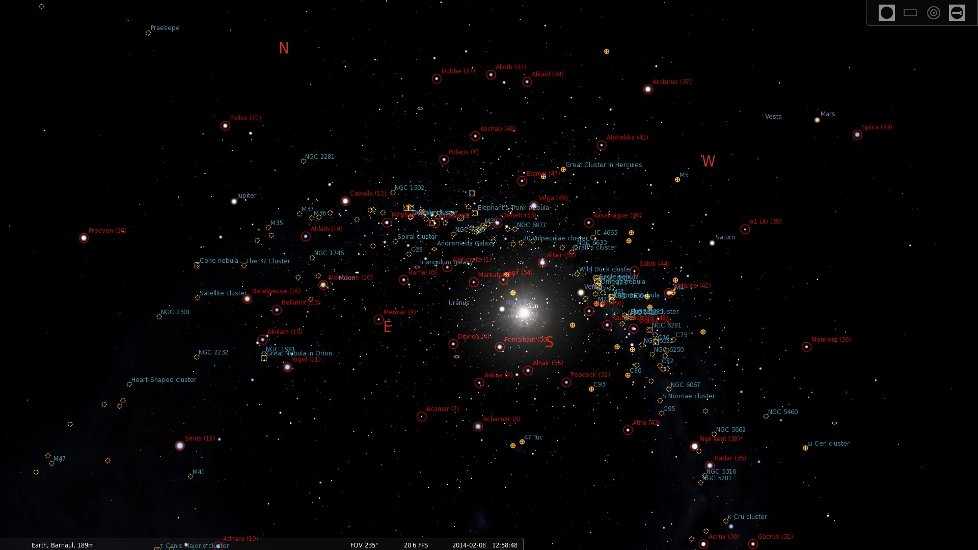
\includegraphics[width=\textwidth]{navstars.jpg}
\caption{Navigational stars on the screen}
\label{fig:plugin:NavigationalStars}
\end{figure}

\noindent This plugin marks navigational stars from a selected set:
\begin{description}
	\item[Anglo-American] --- the 57 "selected stars" that are listed in \emph{The Nautical Almanac}\footnote{The Nautical Almanac
		website -- \url{http://aa.usno.navy.mil/publications/docs/na.php}} jointly published by Her Majesty's Nautical Almanac Office and the US Naval Observatory since 1958; consequently, these stars are also used in navigational aids such as the \emph{2102-D Star Finder}\footnote{Rude Starfinder 2102-D
		description and usage instruction --
		\url{http://oceannavigation.blogspot.ru/2008/12/rude-starfinder-2102-d.html}} and \emph{Identifier}. 
	\item[French] --- the 81 stars that are listed in the \emph{Ephémérides Nautiques} published by the French Bureau des Longitudes.
	\item[Russian] --- the 160 stars that are listed in the Russian Nautical Almanac.
\end{description}
If enabled (see section~\ref{sec:Plugins:EnablingPlugins}), just click
on the Sextant button \guibutton{0.6}{bt_NavStars-off} on
the bottom toolbar to display markers for the navigational stars. This
can help you in training your skills in astronomical navigation before
you cruise the ocean in the traditional way, with your sextant and
chronometer.


\subsection{Section \big[NavigationalStars\big] in config.ini file}
\label{sec:plugins:NavigationalStars:config}

You can edit \file{config.ini} file by yourself for changes of the
settings for the Navigational Stars plugin -- just make it carefully!

\begin{longtabu} to \textwidth {l|l|X}\toprule
\emph{ID}			& \emph{Type} 	& \emph{Description}\\\midrule
navstars\_color 	& R,G,B 		& Color of markers of navigational stars  \\
current\_ns\_set	& string		& Current set of navigational stars. Possible values: \emph{AngloAmerican}, \emph{French} and \emph{Russian}. \\
\bottomrule
\end{longtabu}

\newpage
\section{Satellites Plugin}
\label{sec:plugins:Satellites}

%% GZ: Found on Wiki on 2016-04 with a deprecation note. Still better than nothing!
%% Original URL: http://www.stellarium.org/wiki/index.php/Satellites_plugin
%% TODO: Update from there or write new.

\noindent The Satellites plugin displays the positions of artifical satellites in Earth's orbit based on a catalog of orbital data. It allows
automatic updates from online sources and manages a list of update
file URLs.

To calculate satellite positions, the plugin uses an implementation of
the SGP4/SDP4 algorithms (J.L. Canales' \program{gsat} library), using
as its input data in NORAD's two-line element set
(TLE\footnote{TLE: \url{https://en.wikipedia.org/wiki/Two-line_element_set}})
format. Lists with TLEs for hundreds of satellites are available
online and are regularly updated. The plugin downloads the lists
prepared by \url{http://celestrak.com} to keep itself up-to-date, but the users can
specify other sources online or load updates from local files.

If enabled (see
section~\ref{sec:Plugins:EnablingPlugins}), just click on the
Satellite button \guibutton{0.6}{bt_hint}  on the bottom
toolbar to display markers for the satellites.

It should now be possible to search for artificial satellites using
the regular search dialog (\key{F3}). Note that at any given time, most
Satellites will be below the horizon.

\subsection{Satellite Properties}
\label{sec:plugins:Satellites:properties}

\begin{description}
\item[Name and identifiers] Each satellite has a name. It's displayed as a label of the satellite hint and in the list of satellites. Names are not unique though, so they are used only
for presentation purposes.

\item[Satellite Catalog] In the \emph{Satellite Catalog} satellites are uniquely identified by their NORAD number, which is encoded in TLEs.

\item[Grouping]
A satellite can belong to one or more groups such as ``amateur'',
``geostationary'' or ``navigation''. They have no other function but
to help the user organize the satellite collection.  Group names are
arbitrary strings defined in the Satellite Catalog for each satellite
and are more similar to the concept of tags than a hierarchical
grouping. A satellite may also not belong to any group at all.

By convention, group names are in lowercase. The GUI translates some of the groups used in the default catalog.
\end{description}

\subsection{Satellite Catalog}
\label{sec:plugins:Satellites:catalog}



The satellite catalog is stored on the disk in JSON\footnote{\url{http://www.json.org/}}
format, in a file named \file{satellites.json}. A default copy is embedded in the plug-in at compile time. A working copy is kept in the user data directory.

%   Used in Satellites plug-in 0.7.1 and later (Stellarium 0.11.2 and later) 

To add a new satellite, open a new line after line 5 and paste the following, note commas and brackets, they are important:
\begin{configfile}[\scriptsize]
"NORAD number": 
{
  "name": "name of the satellite"
  "description": "description goes here",
  "comms": [
     {
  	"description": "downlink 1",
  	"frequency": 437.49,
  	"modulation": "AFSK 1200 bps"
     },
     {
  	"description": "downlink 2",
  	"frequency": 145.825
     }
              ],
  "groups": ["group1", "group2"],
  "tle1": "1 12345U 90005D   09080.85236265  .00000014  00000-0  20602-4 0  5632",
  "tle2": "2 12345 98.2700  53.2702 0011918  71.1776 289.0705 14.31818920   653",
  "visible": true
},
\end{configfile}
Explanation of the fields:

\begin{description}
\item[NORAD number]  required parameter, surrounded by double quotes (\texttt{"}),
followed by a colon (\texttt{:}). It is used internally to identify the
satellite. You should replace the text \texttt{"NORAD number"} with the first number on both lines of the TLE set (in this case, \texttt{"12345"}). It must match the number of the satellite in the source you are adding from if you want the TLE to be automatically updated.
\end{description}
The remaining parameters should be listed between two curly brackets and the closing curly bracket must be followed by a comma to separate it from the next satellite in the list:

\begin{description}
\item[name] required parameter. It will be displayed on the screen and used
when searching for the satellite with the Find window. Use the
description field for a more readable name if you like. (The
description field can accept HTML tags such as \texttt{<br/>} (new line), \texttt{<b></b>} (bold), etc.)

\item[description] optional parameter, double quoted. Appears when you click on the satellite \item[comms] optional parameter, square bracketed list of curly bracketed communications information.
\item[groups]  optional parameter, comma separated list of double quoted group names contained in square brackets. Used for grouping satellites in the drop down box on the config (see above)
\item[tle1]  required, line 1 of the TLE, must be contained in double quotes and begin with \texttt{"1~"}
\item[tle2]  required, line 2 of the TLE, must be contained in double quotes and begin with \texttt{"2~"}
\item[visible]  required parameter, set to true if you want to see it, this can be toggled from the configuration window once the satellite is loaded. 
\end{description}
You can edit the tags for a satellite, modify the description and comms data, and even add new satellites. 


\subsection{Configuration}
\label{sec:plugins:Satellites:configuration}


The plug-in's configuration data is stored in Stellarium's main configuration
file.


\subsection{Sources for TLE data}

\begin{description}
\item[Celestrak]\footnote{\url{http://celestrak.com/NORAD/elements/}} used as default update source, it also has TLE lists
  beyond those included by default in Satellite plug-in
\item[TLE.info]\footnote{\url{http://www.tle.info/joomla/index.php}}
\item[Space Track]\footnote{\url{http://www.space-track.org/}} the definitive source, requires signup, operated by
  United States Department of Defense
\end{description}

%%% Local Variables: 
%%% mode: latex
%%% TeX-master: "guide"
%%% End: 

